\documentclass[12pt]{article}
\usepackage[utf8]{inputenc}
\usepackage{amsmath, amssymb, amsthm}
\usepackage{geometry}
\usepackage{graphicx}
\usepackage{xcolor}
\usepackage{tikz}
\usepackage{pgfplots}
\pgfplotsset{compat=1.18}
\geometry{margin=1in}

\newtheorem{theorem}{Theorem}
\newtheorem{corollary}[theorem]{Corollary}
\newtheorem{definition}{Definition}
\newtheorem{example}{Example}
\theoremstyle{definition}

\DeclareMathOperator*{\argmin}{arg\,min}
\DeclareMathOperator{\supp}{supp}

\title{Understanding the Properties of Real Symmetric Polynomial Functions\\
\large Independent Research Project (MA 499)\\
\normalsize Based on ``On the Positivity of Symmetric Polynomial Functions, Part I: General Results'' by Vlad Timofte}
\author{Srinivas Ganesan\\
\small Mentor: Dr. Hoon Hong}
\date{August 10, 2022}

\begin{document}

\maketitle

\section{Description of the Paper}

This paper summarizes and explains the main results from Vlad Timofte's ``On the Positivity of Symmetric Polynomial Functions, Part I: General Results'' \cite{timofte2003}. Timofte's work presents interesting findings about real symmetric polynomials (polynomials in $\mathbb{R}[x_1, x_2, \ldots, x_n]$ such that if any of the variables are interchanged, the same polynomial is obtained), and real symmetric polynomial inequalities.

The main results of Timofte's paper are theorems about certain continuous functions called $(s)$-paths, that are mapped from a closed bounded interval to $\mathbb{R}^n_+$. When these continuous functions are only mapped to a subset of $\mathbb{R}^n_+$, like $M_o(f)$ (see Notation~\ref{def:Mo} for the definition of $M_o(f)$), they can produce some interesting results that will be discussed below in detail.

For my research I will be summarizing all the results of Timofte's paper, explaining them with examples, and discussing potential ideas that can be researched further.

\begin{quote}
\textbf{Note:} This document only summarizes the main results of the paper. All results will be discussed in my Research Expository and my final paper.
\end{quote}

\section{Notations \& Definitions}
\label{sec:notations}

\subsection{Basic Definitions}

\begin{definition}[$\mathbb{R}^n_+$]\label{def:Rn+}
It is the set of all sequences of non-negative real numbers $(x_1, x_2, \ldots, x_n)$.
\[
\mathbb{R}^n_+ := \{x \in \mathbb{R}^n \mid x \geq 0^n\}
\]
\end{definition}

\begin{example}
$(1, 0, 2) \in \mathbb{R}^3_+$.
\end{example}

\begin{definition}[Real Symmetric Polynomials]\label{def:RSP}
Polynomials in $\mathbb{R}[x_1, x_2, \cdots, x_n]$ which remain unchanged when the index of its variables are permuted.
\end{definition}

\begin{example}
$x_1^2 + x_2^2 = x_2^2 + x_1^2 \in \mathbb{R}[x_1, x_2]$.
\end{example}

\begin{definition}[Real Symmetric Polynomial Inequality]\label{def:RSPI}
Let $f(x)$ be a real symmetric polynomial where $x \in \mathbb{R}^n$. A real symmetric polynomial inequality is an inequality of the form:
\[
f(x) \geq 0, \quad f(x) \leq 0, \quad f(x) > 0, \quad f(x) < 0
\]
\end{definition}

\textbf{Note:} The degree of a symmetric polynomial or a real symmetric polynomial inequality is denoted by $d$.

\begin{example}
Let $f(x) = x_1^2 + x_2^2 + x_3^2 + x_1x_2 + x_2x_3 + x_3x_1$.\\
Then $d = \deg(f) = 2$.

Also, we can say that the inequality $f(x) \geq 0$ has degree $d = 2$.
\end{example}

\subsection{Important Notations}

\begin{definition}[$\sum_{d}^{[n]}$]\label{def:Sigma_d}
It is the set of all real symmetric polynomials in $\mathbb{R}^n$ with degree less than or equal to $d$.
\[
\sum_{d}^{[n]} := \left\{f \in \mathbb{R}[x_1, x_2, \ldots, x_n] \,\Big|\, f \text{ is symmetric}, \deg(f) \leq d\right\}
\]
\end{definition}

\begin{example}
Examples of elements in $\sum_{3}^{[2]}$: $x_1^3 + x_2^3$, $x_1x_2$, $x_1 + x_2$.
\end{example}

\begin{definition}[$P_t(x)$]\label{def:Pt}
It is the sum of powers of all the elements of the $n$-tuple $x$.
\[
P_t(x) := x_1^t + x_2^t + \cdots + x_n^t
\]
\end{definition}

\begin{example}
Let $x = (1, 2)$.\\
$P_2(x) = 1^2 + 2^2 = 5$.
\end{example}

\begin{definition}[$\supp(x)$]\label{def:supp}
It is the set of the indices of all the non-zero elements in $x$.
\[
\supp(x) := \{i \in \mathbb{N}^* \mid x_i \neq 0\}
\]
\end{definition}

\begin{example}
Let $x = (1, 0, 1, 3)$.\\
$\supp(x) = \{1, 3, 4\}$.
\end{example}

\begin{definition}[$\nu^*(x)$]\label{def:nustar}
It is the number of distinct non-zero elements in $x$.
\end{definition}

\begin{example}
Let $x = (1, 0, 3, 1, 3)$.\\
$\nu^*(x) = 2$.
\end{example}

\begin{definition}[Additional Notation]\label{def:additional}
\begin{enumerate}
\item[$\alpha$)] $\lfloor x \rfloor$ := The integer part of $x$.
\item[$\beta$)] $a \vee b$ := $\max\{a, b\}$.
\item[$\gamma$)] $a \wedge b$ := $\min\{a, b\}$.
\end{enumerate}
\end{definition}

\subsection{Important Definitions}

Let $\sigma \in \mathbb{R}$, and $\sigma > 0$. Let $s \in \mathbb{N}^*$. Let $f \in \sum_d^{[n]}$.

\textbf{Note:} In the paper $f$ is defined as any continuous function mapped from $\mathbb{R}^n_+ \setminus \{0_n\}$ to $\mathbb{R}$, where $0_n = (0, 0, \ldots, n \text{ times})$. But for our purpose, we take $f \in \sum_d^{[n]}$.

\begin{definition}[$K_{\sigma}$]\label{def:Ksigma}
\[
K_{\sigma} := \left\{x \in \mathbb{R}^n_+ \,\Big|\, x_1 + x_2 + \cdots + x_n = \sigma\right\}
\]
\end{definition}

\begin{example}
Let $\sigma = 5$, $n = 2$.
\[
K_5 = \left\{x \in \mathbb{R}^2_+ \,\Big|\, x_1 + x_2 = 5\right\}
\]

\begin{figure}[h]
\centering
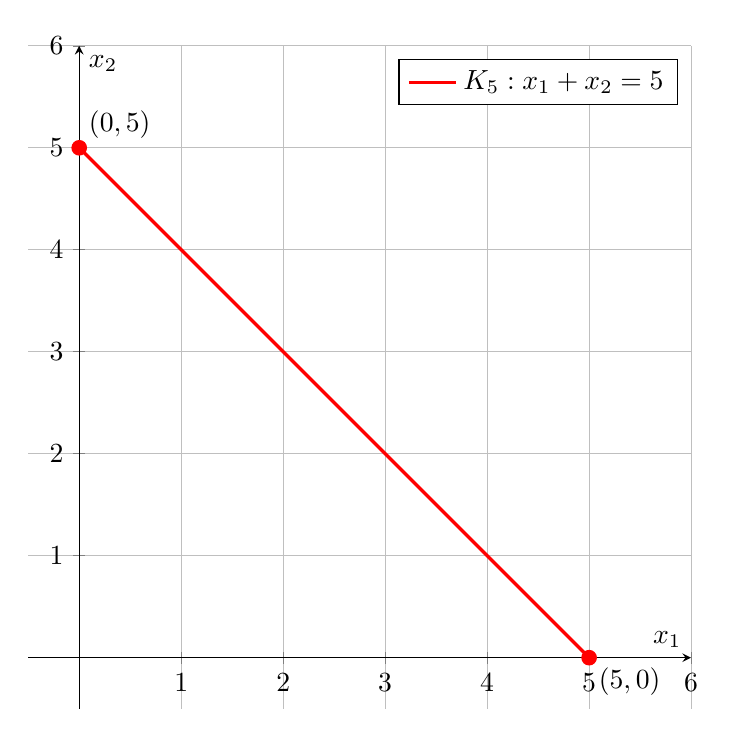
\begin{tikzpicture}
\begin{axis}[
    xlabel=$x_1$,
    ylabel=$x_2$,
    xmin=-0.5, xmax=6,
    ymin=-0.5, ymax=6,
    axis lines=middle,
    width=10cm,
    height=10cm,
    grid=major,
]
% Draw the line x1 + x2 = 5
\addplot[red, very thick, domain=0:5] {5-x};
\addlegendentry{$K_5: x_1 + x_2 = 5$}

% Mark the endpoints
\node[circle,fill=red,inner sep=2pt] at (axis cs:0,5) {};
\node[circle,fill=red,inner sep=2pt] at (axis cs:5,0) {};
\node[above right] at (axis cs:0,5) {$(0,5)$};
\node[below right] at (axis cs:5,0) {$(5,0)$};
\end{axis}
\end{tikzpicture}
\caption{Graph of $K_5$ showing the constraint $x_1 + x_2 = 5$}
\label{fig:K5}
\end{figure}

\vspace{0.5cm}
\end{example}

\begin{definition}[$M_o(f)$]\label{def:Mo}
It is called the minimizer set of function $f$. It is a set that contains all the points in $K_{\sigma}$ that give us the minimum value of $f$.
\[
M_o(f) := \argmin_{x \in K_{\sigma}} f(x)
\]
\end{definition}

\begin{example}
Let $f(x) = x_1x_2$.\\
If we take the example of $K_{\sigma}$ in the previous page,
\[
M_o(f) = \{(0, 5), (5, 0)\}
\]
See Figure~\ref{fig:K5} for a visualization of $K_5$.
\end{example}

\vspace{0.5cm}

\begin{definition}[$(s)$-path, $\gamma: [a, b] \to \mathbb{R}^n$]\label{def:spath}
$\gamma$ is an $(s)$-path if $\gamma$ is a continuous function which satisfies the following conditions:

\begin{enumerate}
\item $\forall t \in [a, b]$, $\forall i$, $1 \leq i \leq s$:
\[
(P_i \circ \gamma)(t) = (P_i \circ \gamma)(a), \quad \text{where } s \in \mathbb{N}^*
\]

\item $\forall t \in [a, b]$:
\[
\supp(\gamma(t)) = \supp(\gamma(a))
\]
\end{enumerate}
\end{definition}

\textbf{Note:} See my exposition for examples of $(s)$-paths.

\vspace{0.5cm}

\section{Main Results}

Throughout this section, we assume the following:
\[
f \in \sum_{d}^{[n]}, \quad \xi \in M_o(f) \text{ for some } \sigma > 0, \quad d \geq 2.
\]

\subsection{Theorem 2.1 (of Enlargement)}
\[
\begin{array}{ccccccc}
\forall n \geq 2 & \forall d \geq 2 & \forall f \in \sum_{d}^{[n]} & \forall \sigma > 0 & \forall \xi \in M_o(f) & \exists & \exists \\
 & & & & \nu^*(\xi) > \lfloor \frac{d}{2} \rfloor & \gamma\text{: injective} & \tilde{\xi} \neq \xi \\
 & & & & & \lfloor \frac{d}{2} \rfloor\text{-path} & \nu^*(\tilde{\xi}) = |\supp(\xi)| \\
 & & & & & \text{in } M_o(f) \cap B(\xi, \varepsilon) & \\
\end{array}
\]
such that $\gamma$ connects $\xi$ to $\tilde{\xi}$.

\subsubsection*{i) Simpler Statement:}

$\forall \xi \in M_o(f)$, $\nu^*(\xi) > L\lfloor \frac{d}{2} \rfloor \Longrightarrow \exists \gamma: [a,b] \to \mathbb{R}^n$, where $\gamma$ is a $L\lfloor \frac{d}{2} \rfloor$-path that injectively maps to a subset of $\mathbb{R}^n$, that is, $M_o(f) \cap B(\xi, \varepsilon)$

$\wedge$

($\gamma$ connects $\xi$ to a point $\tilde{\xi} \in M_o(f)$ s.t $\tilde{\xi} \neq \xi$)

\subsubsection*{ii) Detailed Explanation:}

Let us take a point $\xi = (\xi_1, \xi_2, \ldots, \xi_n) \in M_o(f)$.

If the number of distinct non-zero elements in $\xi$ is greater than the integer part of $\frac{d}{2}$, then for all $\varepsilon > 0$, we can find a $(L\lfloor \frac{d}{2} \rfloor)$-path, that injectively maps to the set $M_o(f) \cap (\varepsilon$-neighborhood of $\xi)$. This $(L\lfloor \frac{d}{2} \rfloor)$-path outputs a point $\tilde{\xi} \in M_o(f) \cap (\varepsilon$-neighborhood of $\xi)$, and $\tilde{\xi} \neq \xi$, which satisfies the interesting condition,
\[
\nu^*(\tilde{\xi}) = |\supp(\tilde{\xi})|
\]

This condition means that all the non-zero elements of $\tilde{\xi}$ are distinct.

\subsubsection*{iii) Purpose of Theorem 2.1:}

The purpose of this theorem is to show an interesting feature of $(s)$-paths.

\subsubsection*{iv) Visual Explanation:}

\fbox{\textbf{See next page}}

To understand Theorem 2.1, we need to understand what the graph of a $L\lfloor \frac{d}{2} \rfloor$-path mapped to $M_o(f) \cap B(\xi, \varepsilon)$ looks like.

\textbf{Note:} The construction of $M_o(f)$ and the $(L\lfloor \frac{d}{2} \rfloor)$-path are not shown for brevity. Also, we take $n = 3$ for the following setting.

\textbf{Legend:}
\begin{itemize}
\item {\color{red}\rule{1cm}{2pt}} $M_o(f)$
\item {\color{green}\rule{1cm}{2pt}} $(L\lfloor \frac{d}{2} \rfloor)$-path
\item {\color{blue}\rule{1cm}{2pt}} $x$ with $\nu^*(x) > L\lfloor \frac{d}{2} \rfloor$
\item {\color{purple}\rule{1cm}{2pt}} $\varepsilon$-neighborhood of $\xi$
\end{itemize}

\textbf{Setting:}
\begin{align*}
f &= x_1 + x_2 + x_3\\
\sigma &= 5\\
K_5 &= \{x : x_1 + x_2 + x_3 = 5\}\\
d &= 3
\end{align*}

\begin{figure}[H]
\centering
\includegraphics[width=0.85\textwidth]{theorem21_graph.pdf}
\caption{Visual representation of Theorem 2.1 showing the relationship between $M_o(f)$, $(L\lfloor d/2 \rfloor)$-paths, and the $\varepsilon$-neighborhood in 3D space}
\label{fig:theorem21}
\end{figure}


\textbf{Note:} The green dotted lines on the red plane indicate that $M_o(f) \subset L\lfloor \frac{d}{2} \rfloor$-path.

\textbf{Observation:} Notice how the $(L\lfloor \frac{d}{2} \rfloor)$-path connects $\xi$ to a point $\tilde{\xi} \neq \xi$, where $\tilde{\xi} \in M_o(f) \cap B(\xi, \varepsilon)$, and all the non-zero elements of $\tilde{\xi}$ are distinct from each other.

\newpage

\subsection{Theorem 2.2 (of Reduction)}
\[
\begin{array}{cccccc}
\forall n \geq 2 & \forall d \geq 2 & \forall f \in \sum_d^{[n]} & \forall \sigma > 0 & \forall \xi \in M_o(f) & \exists \\
 & & & & & \gamma: [a,b] \to \mathbb{R}^n \\
 & & & & & \gamma \text{ is } L\lfloor \frac{d}{2} \rfloor\text{-path} \\
 & & & & & \text{in } M_o(f) \\
\end{array}
\]
\[
\begin{array}{cc}
\exists & \gamma \text{ connects } \xi \text{ to } \tilde{\xi}\\
\tilde{\xi} \in M_o(f) & \\
\nu^*(\tilde{\xi}) \leq L\lfloor \frac{d}{2} \rfloor & 
\end{array}
\]

\subsubsection*{i) Simpler Statement:}

$\forall \xi \in M_o(f)$, $\exists \gamma: [a,b] \to \mathbb{R}^n$ where $\gamma$ is a $L\lfloor \frac{d}{2} \rfloor$-path that connects $\xi$ to a point $\tilde{\xi} \in M_o(f)$ s.t
\[
\nu^*(\tilde{\xi}) \leq L\lfloor \frac{d}{2} \rfloor
\]

\subsubsection*{ii) Detailed Explanation:}

For any point $\xi$ we take, that belongs to the minimizer set of the symmetric polynomial $f$, there exists a continuous function $\gamma$ (a $L\lfloor \frac{d}{2} \rfloor$-path), that connects $\xi$ to a point $\tilde{\xi} \in M_o(f)$ s.t $\nu^*(\tilde{\xi}) \leq L\lfloor \frac{d}{2} \rfloor$.

It should be noted that Theorem 2.2 (and Theorem 2.1) revolve around finding a $L\lfloor \frac{d}{2} \rfloor$-path to ``connect'' $\xi$ to $\tilde{\xi}$. This is because, using a $L\lfloor \frac{d}{2} \rfloor$-path to find a point $\tilde{\xi}$ ensures that $\tilde{\xi}$ lies on a $L\lfloor \frac{d}{2} \rfloor$-path, and therefore has important properties of a point that lies on a $L\lfloor \frac{d}{2} \rfloor$-path (in addition to the properties stated in the claim, like, $\nu^*(\tilde{\xi}) \leq L\lfloor \frac{d}{2} \rfloor$ in Theorem 2.2), like:

\begin{enumerate}
\item[a)] $P_i(\tilde{\xi}) = (P_i \circ \gamma)(a)$, $\forall i \in \mathbb{N}^*$ s.t $1 \leq i \leq L\lfloor \frac{d}{2} \rfloor$
\item[b)] $\supp(\tilde{\xi}) = \supp(\gamma(a))$
\end{enumerate}

\textbf{Note:} i) $\gamma: [a,b] \to \mathbb{R}^n$ is the $L\lfloor \frac{d}{2} \rfloor$-path used above.

\hspace{1.3cm} ii) Since $\xi$ also belongs to the $L\lfloor \frac{d}{2} \rfloor$-path (similar to the point $\tilde{\xi}$), we know that:
\begin{enumerate}
\item[a)] $P_i(\xi) = P_i(\tilde{\xi}) = (P_i \circ \gamma)(a)$, $\forall i \in \mathbb{N}^*$ s.t $1 \leq i \leq L\lfloor \frac{d}{2} \rfloor$
\item[b)] $\supp(\tilde{\xi}) = \supp(\xi) = \supp(\gamma(a))$
\end{enumerate}

\subsubsection*{iii) Purpose of Theorem 2.2:}

The purpose of Theorem 2.2 is to find a point $\tilde{\xi}$, for every $\xi \in M_o(f)$, that satisfies several interesting properties.

\textbf{Note:} The graphical representation of Theorem 2.2 is very similar to the graph that I have drawn for Theorem 2.1. Therefore, I have excluded it from my summary.

\newpage

\subsection{Corollary 2.1}

\subsubsection*{i) Concise Statement of the Corollary:}

\begin{enumerate}
\item[(1)] A symmetric polynomial inequality of degree $d \in \mathbb{N}^*$ holds on $\mathbb{R}_+^n$ 
\[
\Longleftrightarrow
\]
The symmetric polynomial inequality holds on $\{\xi \in \mathbb{R}_+^n \mid \nu^*(x) \leq L\lfloor \frac{d}{2} \rfloor \vee 1\}$.

\item[(2)] A symmetric polynomial inequality of even degree $d \in \mathbb{N}^*$ holds on $\mathbb{R}^n$ 
\[
\Longleftrightarrow
\]
The symmetric polynomial inequality holds on $\{\xi \in \mathbb{R}^n \mid \nu(x) \leq (\frac{d}{2}) \vee 2\}$.
\end{enumerate}

\subsubsection*{ii) Detailed Explanation:}

Based on its definition, symmetric polynomial inequalities are always of the form:
\[
f(x) \geq 0, \quad f(x) \leq 0, \quad f(x) > 0, \quad f(x) < 0
\]

These inequalities can also be interpreted as having the form:
\[
f(x) \geq 0, \quad g(x) \geq 0, \quad f(x) > 0, \quad g(x) > 0 \quad \text{(where } g(x) = -f(x)\text{)}
\]

In other words, by rearranging every symmetric polynomial inequality into the form $f(x) \geq 0$ or $f(x) > 0$, the question ``where does the symmetric polynomial inequality hold?'' can be reinterpreted as ``Over what region is the value of the symmetric polynomial $f(x)$ POSITIVE?''.

This reinterpretation helps us understand why the original research paper is titled ``On the POSITIVITY of Symmetric Polynomial Functions''.

Corollary 2.1 is useful because it provides us with a really easy way to check if a symmetric polynomial inequality holds on the entire $n$-dimensional space $\mathbb{R}_+^n$ (and $\mathbb{R}^n$ as well for inequalities of even degree). It does this by reducing the region where the inequality needs to be evaluated, from $\mathbb{R}_+^n$ to a much smaller set $\{\xi \in \mathbb{R}_+^n \mid \nu^*(x) \leq L\lfloor \frac{d}{2} \rfloor \vee 1\}$. To check if a symmetric polynomial inequality of EVEN degree holds on entire $\mathbb{R}^n$, as well, we only need to evaluate the inequality on a much smaller subset of $\mathbb{R}^n$, that is, $\{\xi \in \mathbb{R}^n \mid \nu(x) \leq (\frac{d}{2}) \vee 2\}$.

Corollary 2.1 provides us with an interesting relationship between the region where a symmetric polynomial inequality holds, and the number of distinct non-zero elements $(\nu^*(x))$ in the points in that region.

\subsubsection*{iii) Example:}

Let $n = 2$, $d = 2$.

Symmetric Polynomial inequality of degree $d = 2$ \& $n = 2$:
\[
x_1 + x_2 - x_1x_2 < 0 \qquad \Longleftrightarrow \qquad x_1x_2 - x_1 - x_2 > 0
\]

We can observe that,
\[
L\lfloor \frac{d}{2} \rfloor \vee 1 = L\lfloor 1 \rfloor \vee 1 = 1, \quad \text{and} \quad L\lfloor \frac{d}{2} \rfloor \vee 2 = \frac{2}{2}
\]

Assume $A := \{x \in \mathbb{R}_+ \mid \nu^*(x) \leq L\lfloor \frac{d}{2} \rfloor \vee 1\}$
\[
= \{x \in \mathbb{R}_+ \mid \nu^*(x) \leq 1\}
\]

\textbf{Example elements in $A$:}
\begin{center}
\begin{tabular}{ccccc}
$(1,1)$ & $(1,0)$ & $(\sqrt{2}, \sqrt{2})$ & $(0, 1.5)$ & $(0,0)$ \\
$\downarrow$ & $\downarrow$ & $\downarrow$ & $\downarrow$ & $\downarrow$ \\
$\nu^*(x) = 1$ & $\nu^*(x) = 1$ & $\nu^*(x) = 1$ & $\nu^*(x) = 1$ & $\nu^*(x) = 0$
\end{tabular}
\end{center}

Now let us observe how Corollary 2.1 is used, through a graphical representation of the inequality.

\textbf{Legend:}
\begin{itemize}
\item \colorbox{green!50}{\ \ \ \ \ } Region where the inequality holds.
\item {\color{red}\rule{1cm}{2pt}} Set $A$
\item {\color{blue}\rule{1cm}{2pt}} Subset of set $A$, where the inequality fails.
\end{itemize}

\textbf{Note:} The {\color{blue}BLUE} line lies on the {\color{red}RED} line.

\textbf{Graph:}
\begin{figure}[h]
\centering
\includegraphics[width=0.85\textwidth]{corollary_graph.pdf}
\caption{Graphical representation showing that the inequality $x_1x_2 - x_1 - x_2 > 0$ does not hold on all of $\mathbb{R}_+^2$ by examining set $A$}
\label{fig:corollary21example}
\end{figure}

Since the inequality doesn't hold on the points lying on the blue line, the inequality does not hold for all elements of set $A$.

$\Rightarrow$ Therefore, the inequality does not hold on $\mathbb{R}_+^2$.

\vspace{1cm}

\textbf{Note:} An example for the (2) result of Corollary 2.1 will be very similar to the example shown in the previous page (for (1) result of Corollary 2.1).

\clearpage

\section{Conclusion of Summary}

To conclude, this paper shows how symmetricity of a polynomial (and even functions other than polynomials) can give the polynomial (or function) several interesting properties that are absent in normal (asymmetric) polynomials.

\bibliographystyle{plain}
\begin{thebibliography}{9}

\bibitem{timofte2003}
V. Timofte,
\textit{On the positivity of symmetric polynomial functions. Part I: General results},
Journal of Mathematical Analysis and Applications,
vol. 284, no. 1, pp. 174--190, 2003.

\end{thebibliography}

\end{document}